%%% The ``\documentclass'' command has one parameter, based on the kind of
%%% document you are preparing.
%%%
%%% [annual] - Technical paper accepted for presentation at the ACM SIGGRAPH 
%%%   or SIGGRAPH Asia annual conference.
%%% [sponsored] - Short or full-length technical paper accepted for 
%%%   presentation at an event sponsored by ACM SIGGRAPH
%%%   (but not the annual conference Technical Papers program).
%%% [abstract] - A one-page abstract of your accepted content
%%%   (Technical Sketches, Posters, Emerging Technologies, etc.). 
%%%   Content greater than one page in length should use the "[sponsored]"
%%%   parameter.
%%% [preprint] - A preprint version of your final content.
%%% [review] - A technical paper submitted for review. Includes line
%%%   numbers and anonymization of author and affiliation information.

\documentclass[annual]{acmsiggraph}

%%% If you are submitting your paper to one of our annual conferences - the 
%%% ACM SIGGRAPH conference held in North America, or the SIGGRAPH Asia 
%%% conference held in Southeast Asia - there are several commands you should 
%%% consider using in the preparation of your document.

%%% 1. ``\TOGonlineID''
%%% When you submit your paper for review, please use the ``\TOGonlineID''
%%% command to include the online ID value assigned to your paper by the
%%% submission management system. Replace '45678' with the value you were
%%% assigned.

\TOGonlineid{}

%%% 2. ``\TOGvolume'' and ``\TOGnumber''
%%% If you are preparing a preprint of your accepted paper, and your paper
%%% will be published in an issue of the ACM ``Transactions on Graphics''
%%% journal, replace the ``0'' values in the commands below with the correct
%%% volume and number values for that issue - you'll get them before your
%%% final paper is due.

\TOGvolume{0}
\TOGnumber{0}

%%% 3. ``TOGarticleDOI''
%%% The ``TOGarticleDOI'' command accepts the DOI information provided to you
%%% during production, and which makes up the URLs which identifies the ACM
%%% article page and direct PDF link in the ACM Digital Library.
%%% Replace ``1111111.2222222'' with the values you are given.

\TOGarticleDOI{1111111.2222222}

%%% 4. ``\TOGprojectURL'', ``\TOGvideoURL'', ``\TOGdataURL'', ``\TOGcodeURL''
%%% If you would like to include links to personal repositories for auxiliary
%%% material related your research contribution, you may use one or more of
%%% these commands to define an appropriate URL. The ``\TOGlinkslist'' command
%%% found just before the first section of your document will add hyperlinked
%%% icons to your document, in addition to hyperlinked icons which point to
%%% the ACM Digital Library article page and the ACM Digital Library-held PDF.

\TOGprojectURL{}
\TOGvideoURL{}
\TOGdataURL{}
\TOGcodeURL{}

%%% Replace ``PAPER TEMPLATE TITLE'' with the title of your paper or abstract.

\title{Medipa: Visualizing Medical Scans in 3D on the Web}

%%% The ``\author{}'' command takes the names and affiliations of each of the
%%% authors of your paper or abstract. The ``\thanks{}'' command takes the
%%% contact information for each author.
%%% For multiple authors, separate each author's information by the ``\and''
%%% command.

\author{Juhee Bae\thanks{e-mail: jbae3@ncsu.edu}\\ North Carolina State University %
\and Eric D. Helms\thanks{e-mail: edhelms@ncsu.edu}\\North Carolina State University}

%%% The ``pdfauthor'' command accepts the authors of the work,
%%% comma-delimited, and adds this information to the PDF metadata.

\pdfauthor{Juhee Bae, Eric D. Helms}

%%% Keywords that describe your work. The ``\keywordlist'' command will print
%%% them out.

\keywords{Volume Rendering, WebGL, Medical Images}

%%% The ``\begin{document}'' command is the start of the document.

%%% If you have user-defined macros, you may include them here.

% example of a user-defined macro called ``remark.''
% \newcommand{\remark}[1]{\textcolor{red}{#1}}

\begin{document}

%%% A ``teaser'' image appears under the title and affiliation information,
%%% horizontally centered, and above the two columns of text. This is OPTIONAL.
%%% If you choose to have a ``teaser'' image, it needs to be placed between
%%% ``\begin{document}'' and ``\maketitle.''

%\teaser{
%   \includegraphics[height=1.5in]{images/sampleteaser}
%   \caption{Spring Training 2009, Peoria, AZ.}
%}

%%% The ``\maketitle'' command must appear after ``\begin{document}'' and,
%%% if you have one, after the definition of your ``teaser'' image, and
%%% before the first ``\section'' command.

%%% Your paper's abstract goes in its own section.

\teaser{
	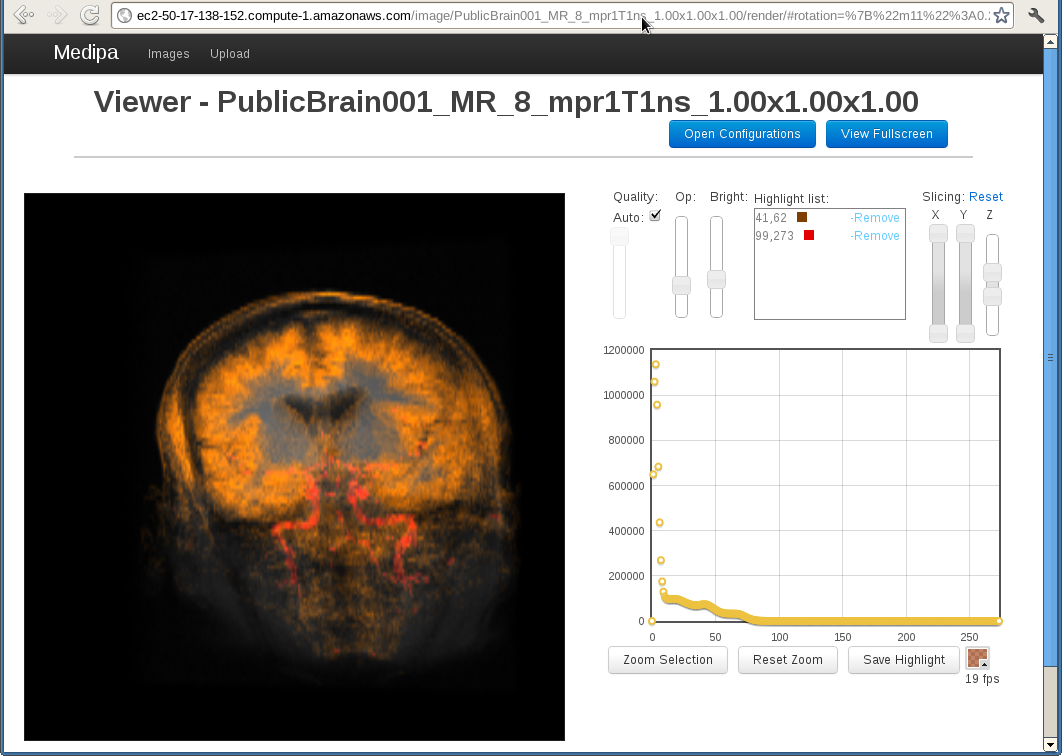
\includegraphics[scale=0.45]{head.png}
	\caption{\label{fig:head}Brain rendered with Medipa}
}

\maketitle

\begin{abstract}
We introduce Medipa, an open-source system to render medical images on the web in 3D that allow multiple medical representatives to investigate, analyze and annotate a single image.  A user can  upload medical image scans, adjust the zoom level, select pixels and highlight them, slice the volume.  Further, to harness the distributed nature of the web and provide a tool for collaboration users can save configurations that consist of the aforementioned adjustable properties and add comments. The rendering algorithm is based on volume ray-tracing using shaders implemented in WebGL, Javascript, and HTML5.
\end{abstract}
%%% ACM Computing Review (CR) categories.
%%% See <http://www.acm.org/class/1998/> for details.
%%% The ``\CRcat'' command takes four arguments.

\begin{CRcatlist}
  \CRcat{I.3.7}{Computer Graphics}{Three-Dimensional Graphics and Realism}{Radiosity};
\end{CRcatlist}

%%% The ``\keywordlist'' command prints out the keywords.

\keywordlist

%%% The ``\TOGlinkslist'' command will insert hyperlinked icon(s) to your
%%% paper. This includes, at a minimum, hyperlinked icons to the ACM article
%%% page and the ACM Digital Library-held PDF. If you added URLs to
%%% ``\TOGprojectURL'' or the other, similar commands, they will be added to
%%% the list of icons.
%%% Note: this functionality only works for annual-conference papers.

\TOGlinkslist

%%% The ``\copyrightspace'' command 
%%% Do not remove this command.

\copyrightspace

%%% This is the first section of the body of your paper.

\section{Introduction}
The current state of the art for viewing medical image scans requires using a desktop application.  This means having the software installed on every computer a medical health practitioner wishes to view the scans on as well as ensuring that computer runs the required operating system and has the required packages installed.  Further, these systems are geared towards viewing and recording information based on scan analysis not on collaborative efforts.

As web browser technology has evolved, access to the underlying GPU and APIs that follow the OpenGL standard have been added for doing complex 2D and 3D rendering.  This allows for the creation of complex applications using the browser as a platform that used to require a full desktop application.  The web provides a platform that is operating-system agnostic and allows users to use their favorite browser for interaction.  Further, by serving the content up from a central location, users can go anywhere in the world and still have access to viewing the scans.  This opens up a world where scans can be viewed by a variety of people and crowd-sourcing of ideas can be shared.

The rise of social media interaction, and distributed interaction of users has begun to spill over in to every field.  Further, as the availability of information increases and more and more users take responsibility of their personal data, the desire for people to want to see their medically relevant health information will rise.  By harnessing the web, data that has never been available at a personal level or able to be collaborated on can begin to flourish.  The MedIPA system aims to take a first step in this direction by providing volume rendered medical scans uploaded by users that can be manipulated, saved and commented on in order to procure a dialog.  In this way, users can view their own medical scans, share it with others, or seek further opinions on aspects of the images.  The same goes for medical professionals.

The appearance of HTML5 enables high quality drawing, provides flexible controls, and enhances the visual appearance of the web interface. Volume rendering was one of the challenges that users wanted to see on the web with interaction. Volume rendering is to display 3D scalar field dataset to a 2D image, but the computation time and memory load are the overhead. In this study, we demonstrate volume rendering of medical images on the web using volume ray-casting with HTML5. We also allow the users to save the configuration to keep history of the rendered image and to share and collaborate the result with others. 

The rest of the paper is organized as follows: Section 2 provides a look at related works in the area of volume rendering, Section 3 talks about the concept, Section 4 covers details of the implementation, Section 5 discusses limitations, Section 6 discusses possible future work and Section 7 finishes with conclusions.


\section{Related Works}
The technique of volume rendering gained a lot of interest especially to investigate medical data. The process of volume rendering has several stages to produce the result image \cite{drebin:1988}. First, the input volume data set is converted to a set of material percentage volumes. Each element in the volume is called a voxel (volume element) which the value represents the percentage of the material in a region of space. After classifying the dataset, a linear ramp called a transfer function assigns the opacity and color values to every voxel in the volume. It allows viewing a certain part of the volume by selecting a certain range of opacity and color. Next, the volume is projected to the image plane by compositing the opacity and colors of the voxels. 

Previous researches attempted multiple methods to visualize volumes. Marching cubes \cite{lorensen:1987} provided an algorithm that creates polygonal representation of iso-surfaces from a three dimensional array of data. It uses a table of possible edge intersections of a cube which describes how a surface cuts the surface. For realism, it calculates the normalized gradient from the original data which helps to create the desired surface model. However, the drawback of the algorithm is the speed regarding to the great number of triangles and overhead by rotation. The amount of memory needed for the surface result is another problem. Also, there exists a hole problem which you see a hole of the result image when at least one cube face has an intersection point in each of its four edges.

Levoy\cite{levoy:1990} introduced an efficient way to use ray-tracing for volume rendering. It improves its performance by employing binary volumes of coherent regions and adaptively terminating ray-tracing at the user-selected opacity threshold. However, the method is not interactive.
For interactivity, splatting provided a way to perform volume rendering in parallel. It is a technique that splats every voxel to the viewing surface in back-to-front order as if throwing a snow ball to a wall \cite{westover:1991}. This method runs in parallel, thus reduces the rendering time, but produces respectively lower image qualities. 
Recently, interesting work on WebGL have been conducted with volume rendering \cite{anatomical:2011}. 


\section{Concept}
	The solution provided by the MedIPA system focused on a two phase approach.  The first phase takes medical scans in their binary input format and processes them.  This processing is designed to turn the binary formats into a usable format when rendered in the browser and produce reductions of the data to provide lower quality images for faster loading and ease of user interaction.  The second phase involves taking the raw processed 2-dimensional data and rendering it within the browser as a volume.  The second involved two different approaches due to the first approach taken becoming unfeasible at scale.  The next three sub-sections describe the data processing phase and both attempts at 3D rendering.

\subsection{Data Processing}

Most medical image scans come in a binary format that can not be directly ported to WebGL for rendering.  Given this limitation, a small data processing library was created taking advantage of SimpleITK.  SimpleITK is a library that can turn binary format medical scans into data representations that can be worked on within native code.  The layer would take in the binary medical scan format, process with SimpleITK and then turn the outputted pixel data array into a series of PNG's that represented each layer of the scan.  The subsequent PNG is saved down to the file system along with a JSON based file that contains metadata about the image.  This metadata included filenames, dimensions, configuration information and pixel histogram information.

Given that some systems may be limited in their graphical processing power, down sampling of the image resolution was added to the data processing layer.  Whenever an image is processed by the server, the data points are reduced 3 times and for each reduction a PNG is saved off and entry made into the manifest file.  The reductions occur by selecting an octet of the pixels and finding an average location and value.  This produces images that are 1/8, 1/64 and 1/512 the size and dimensions of the original image scan.

Down sampling the image provides two direct benefits that are related to the reliance on the client to handle rendering of the data.  The first benefit comes from being able to reduce the size of the image bundle being sent across the wire.  Low resolution images translate to small file sizes.  This in turn means that when the user first accesses the render page a small image can be sent quickly across for the user to start viewing and interacting automatically.  As time progresses, the system can fetch higher resolution images and swap them in behind the scenes for the user to allow continued interaction without interruption.  

The second benefit comes from the variability in client computer graphics processing power.  Attempting to render high resolution images on an under powered machine can not only place the application into an unusable state but also render the entire client machine unusable by the user as the CPU and GPU attempt to handle the large resolution.  Thus, having lower resolution images helps to allow users with under powered machines to still interact with the system.  Further, the client code monitors the frames-per-second (FPS) as each data resolution is brought in and will halt the quality increases if the code determines that the system would enter an unusable state.

\subsection{Marching Cubes}
	The marching cubes algorithm....
	This algorithm was implemented in the browser by creating a set of parallel Web Workers that each processed a different portion of the image array data.  Originally, the workers would each ask the server for the data set which introduced a lot of network traffic and redundant memory allocation.  Further improvements loaded the data set once and passed it to the workers.  Each worker processed independently and sent a signal with the return data back to a centralized worker queue.  Once all workers had finished the rendering algorithm took the results and generated the iso-surfaces.  
	The test bed system had 4GB of memory, a 2.3GHZ dual-core, hyper-threaded processor using 8 Web Workers.  For small data-sets (less than 500KB), the algorithm finished and rendered within a reasonable amount of time (< 1 second).  As the data began to scale in size, the computation time for the Marching Cubes algorithm increased to an unusable level capping out at a 25 minute calculation time for a 2.3MB set which roughly equated to over 1 million points.  Further, it became evident that the Marching Cubes approach would not allow for users to treat the rendered volume as a slice-able entity.

\subsection{Rendering algorithm}
	Volume rendering displays 3D scalar field dataset to a 2D image. The two traditional ways are slice-based rendering and volume ray tracing. Our algorithm follows volume ray tracing that shoots rays through the volume and samples along the path by equal intervals. As the sampling points are advanced along the ray, it accumulates the opacity and RGB values of the sampling points. By the use of transfer function, it assigns the color and opacity values to each voxel in the volume and shows the corresponding emission and absorption of light for the sample point. The transfer function enables to observe a specific part of the volume given the range of the density value in the dataset. We allowed easier interaction with the visual controls to manipulate the range of the dataset as well as the color and opacity values on the client side. 
The advantages of ray tracing are optimization from empty space skipping, independence of the projection view, and easiness of development. In order to improve performance, the algorithm renders the position of front and back facing triangles to the textures instead of calculating the intersection between the ray and the bounding box around the volume. The front face texture provides the start position of the ray and the result of subtracting from back to front face texture provides the direction of the ray. Then, starting from the start position of each ray, the algorithm accumulates the color and opacity value of the sampling point in front-to-back direction in parallel. In addition, the process is optimized to stop earlier when the accumulated opacity reaches to the maximum value (i.e.,1.0) or when the advance of ray tracing reached the length of the ray. It is possible by the back face texture which contains the end position of the ray for each pixel. The code is shown below.



$vec3 raystart = v_PosLocal; \\
vec2 texcoords = (v_Position.xy / v_Position.w + vec2(1.0, 1.0)) / 2.0; \\
vec3 rayend = texture2D(backpos_tex, texcoords).xyz; \\
vec3 raydir = rayend - raystart; \\
vec3 deltadir = normalize(raydir) * stepsize; \\
float len = length(raydir); \\
float deltadirlen = length(deltadir); \\
vec3 raypos = raystart + steps * interstep * deltadir; \\
float lengthsum = steps * interstep * deltadirlen; \\
vec4 colorsum = mix(vec4(0.0, 0.0, 0.0, 0.0), texture2D\\(intermediate_tex, texcoords), clamp(interstep, 0.0, 1.0)); \\
vec4 colorsample; \\
\\
for (float i = 0.0; i < steps; i += 1.0) \{ \\
	if (lengthsum >= len || colorsum.a >= 1.0) break; \\
	colorsample = tex3D(raypos); \\
	colorsample.a *= stepsize * opacity; \\
	colorsum.rgb += colorsample.rgb * colorsample.a * (1.0 - colorsum.a); \\
	colorsum.a += colorsample.a * (1.0 - colorsum.a); \\
	raypos += deltadir; \\
	lengthsum += deltadirlen; \\
\} \\
\\
gl_FragColor = mix(colorsum, vec4(colorsum.rgb * \\clamp(colorsum.a, 0.0, 1.0) *  brightness, 1.0), finalstep); $\\


We used WebGL, javascript, and HTML5 for implementing volume ray tracing. We also refered to previous work performed on volume rendering with WebGL \cite{anatomical:2011}. The details are described in the following section about the system. 

\begin{figure*}[htb]
	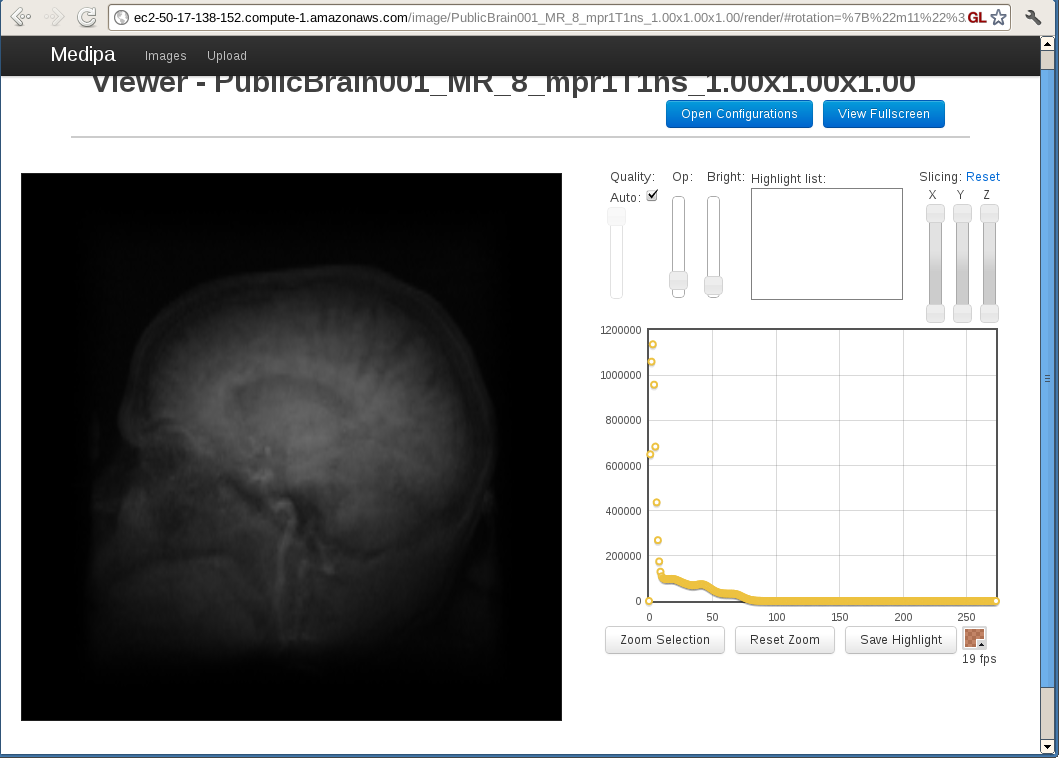
\includegraphics[scale=0.475]{clean_interface.png}
	\caption{\label{fig:head}Basic interface with no modifications}
\end{figure*}

\section{Architecture}
	The Medipa system was designed in order to allow users to upload or post URLs of medical image scans in their native formats, have them processed by an asynchronous task queue and provide an interactive rendering page for viewing the image scans as volume data.  Further, the rendering interaction provides users with tools to examine, modify and save user defined configurations of the rendered data.  The underlying system was designed as a web-based Model-View-Controller (MVC) pattern with a data processing layer server side, asynchronous task queue and all rendering happening within the user's browser.  The architecture can be seen in Figure 3.

\begin{figure*}[htb]
	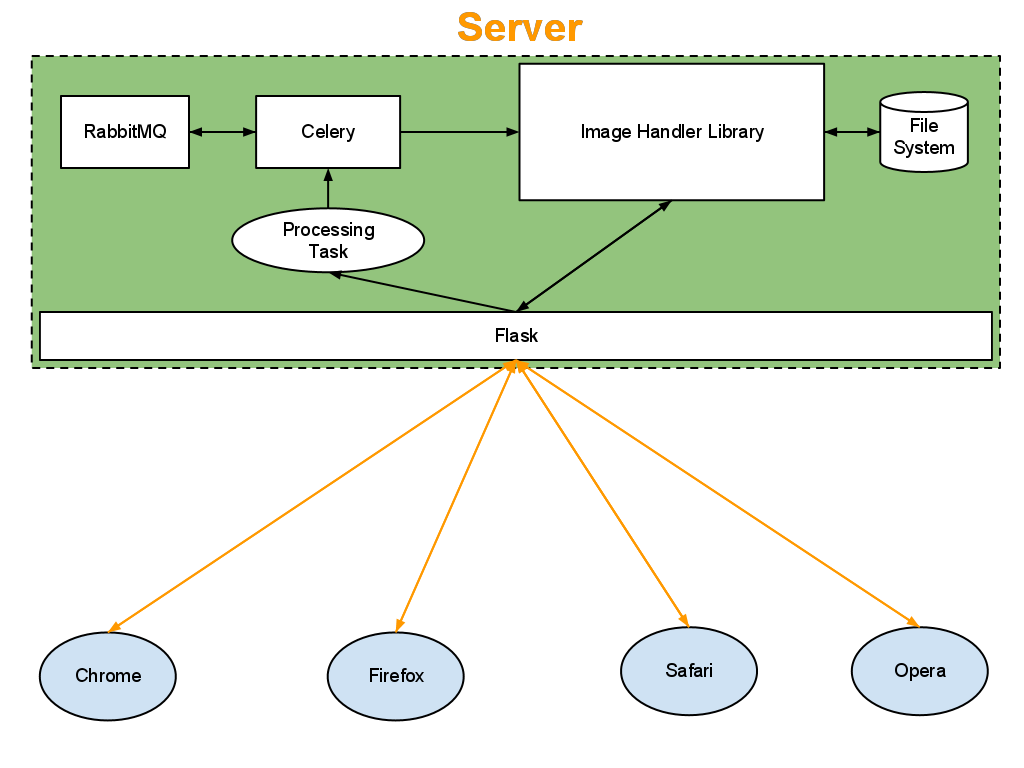
\includegraphics[scale=0.475]{architecture.png}
	\caption{\label{fig:head}MedIPA System Architecture}
\end{figure*}

\subsection{Server}
	The server uses the Python micro web-framework Flask to create a set of urls and associate controllers for each.  Using the Jinja2 templating language, a series of templated HTML files that act as the views are associated with each controller action.  The model layer is handled by an image processing library that stores files to disk and uses a JSON formatted manifest file to store relevant data and references to files stored on disk.  Any call to retrieve or store data is processed through this library.

\subsubsection{Model Layer}
	The model layer is represented by a simple NoSQL JSON schema that is stored directly to the file system and accessed by a small library.  For each uploaded file, a JSON file is created that stores the location of the original file, pre-computed histogram data, configuration data and an entry for each reduced dataset.  Configurations are represented by a unique name that acts as an identifier.  This identifier acts a key in the key-value store for configurations.  Each configuration contains an HTTP GET style parameter list and associated comment from a user.  For each image reduction performed by the data processing layer, a new PNG is saved to disk, and metadata such as the dimensions and filename are stored within the model.

\subsubsection{Controller Layer}
	The controller layer, represented by the Flask box in Figure, provides a thin web handling layer for declaring URLs and associating a function to handle each URL.  The URLs serve to provide a RESTful API and each underlying function hands off work to the image library.

\subsubsection{View Layer}
	The view layer is handled by a combination of a template engine, HTML and Javascript.  The view layer uses the Jinja2 template engine to create view snippets that inherit from a base layout in order to reduce repetition and make creating similarly styled pages easier.  The template handles laying out the structural page layout while Javascript is used to handle initializing of widgets, data retrieval and rendering.

\begin{figure*}[htb]
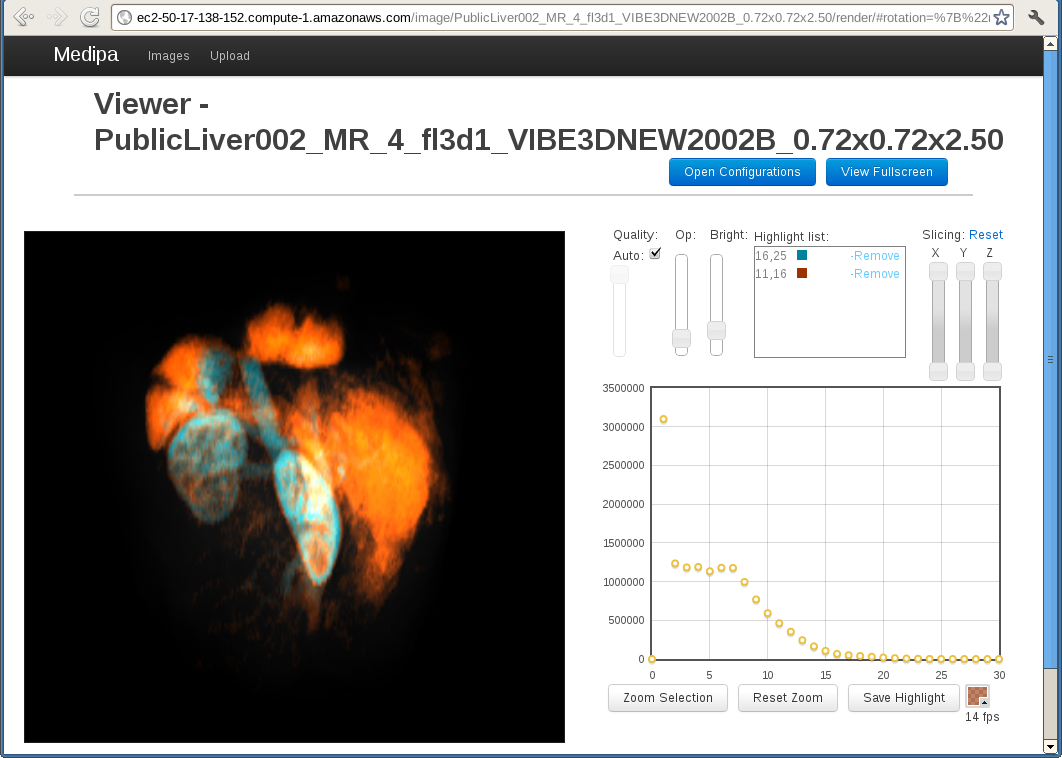
\includegraphics[scale=0.475]{kidneys.png}
	\caption{\label{fig:head}Highlighted Kidney}
\end{figure*}

\subsection{Client Side}
We allow uploading custom image files (e.g., CT, MRI) or from urls. We provide interactive tools to zoom-in, zoom-out, highlight, and slice the volume. Zooming in and out the volume is enabled by manipulating the wheel control of a mouse. In order to select a specific range of the dataset, we display a histogram of the distribution of the density values of the dataset. The user can select a range by drag-and-drop interaction on the histogram and specify a point-of-interest of the volume data. The reason we use a histogram visualization is to see highly concentrated ranges that can be considered interesting regions of the data. It also ables to zoom in and out of the histogram by the x-axis to micro-select the range of the user's point of interest given the distributed values of the data. After the range selection, the user may choose a color to highlight the interested part on the image. The highlighted colors are listed and can be reordered by drag-and-drop interaction. In order to view inside the volume, the interface provides slider widgets to slice the volume on x, y, z axis, independently. In addition, since the tool is expected to share images, to be examined by multiple medical representatives, and commented when necessary, we provide a feature to save the current configuration and comments. The saved configurations can be loaded any time if a particular rendered image needs to be reviewd again. For performance adaptivity on different devices, we allow auto adjustment of image quality. The user can also control the opacity and brightness of the image when needed. The client is accessible online \footnote{available at \url{http://ec2-50-17-138-152.compute-1.amazonaws.com/image/}}.

\subsubsection{Highlighting}
	The highlighting mechanism allows a user to enhance the typical greyscale image to illuminate areas that may not otherwise be obvious.  As a user interacts with the 3D image, particular areas or sections may be highlighted for further investigation or to reference as part of a saved and annotated configuration.  The interaction occurs by highlighting sections of the provided histogram.  The histogram is generated by making counts of all pixels with the same greyscale value display counts on the y-axis and greyscale value on the x-axis.  The user may select a region to be highlighted or to zoom in for higher granularity when selecting particular values to highlight.  
	Discussions with practitioners indicated that seeing these values in a graph format would allow them to look for abnormalities which could then be singled out via highlighting for closer investigation.  By providing a robust color picker, indicated by the color square below the graph, users can even hide portions of the image by selecting a region and setting the alpha channel to zero.  This in turn could allow certain portions, such as a kidney to be highlighted while hiding the rest of the torso similar to Figure 4.
	
\subsubsection{Quality Adjustment}
	As previously discussed, when an image is uploaded and processed the underlying image library generates reduced datasets.  As the page is loaded the image is loaded and processed starting with the low quality image for speed of rendering and user experience.  The quality adjustment tool will, by default, automatically control this interaction by requesting the next dataset size and swapping out the rendering once loaded.  The user is given the option to turn the auto-quality scale off and choose the image quality they desire.  This is done for two reasons.  
	First, the quality of the image loaded is based off the calculated framerate.  In other words, if the framerate drops below a certain threshold (~10 frames-per-second) the image loader will halt and leave the user in a state that is considered usable.  This is done to prevent the users system from becoming unusable by an image quality that would tax the system resources and to allow the user to be able to interact with the system.
	Secondly the user may decide that they desire a higher quality image despite how it may impact their ability to interact.  Thus, the user is presented with the ability to turn off auto-quality adjustments and interact with a slider that will let them select an image quality.

\subsubsection{Zooming}
Zooming is a widely used technique in visualization ~\cite{shneiderman:1996}~\cite{cockburn:2008}. It enables a user to magnify (zoom-in to the point of interest) or demagnify (zoom out to have a brief overview). With the mouse wheel control, we provide smooth zoom-in and zoom-out interaction of the image on the interface. As mentioned in the highlighting section, we also applied zooming to interact with the histogram in order to select a range of interesting greyscale value. It solves the problem of the confliction between the large scaled dataset and the limited space. We also have a button to reset the zooming effect since previous survey has found that zoom-in technique needs to be used in caution when performing region selection. This is because there is no equivalent action for zooming out ~\cite{cockburn:2008}.

\subsubsection{Slicing}
In order to probe the volume data set better, we provide controls to slice the volume. By slicing the volume, it filters out uninteresting part of the volume and reveals the point of interest. We allow users to slice the volume perpendicular to the three dimensions of x, y, and z axis. The slider controller enables the slicing action and resets to the original view by clicking on the reset button. The corresponding interaction technique for slicing is filtering ~\cite{shneiderman:1996}~\cite{yi:2007}. Filtering changes the set of data to be presented based on user-specified conditions. 

\subsubsection{Rotation}
Rotating an object is now a generally common interaction technique in visualization. It is one of the methods to explore the data ~\cite{yi:2007}. Explore enables the users to examine a different subset of the data that is hidden or not displayed at the moment. Rotation allows to easily manipulate which region of volume data to be presented.

\section{Limitations}
Given that typical medical image scans consist of multiple high resolution slices, processing of the image data is resource intensive task.  While the system takes measures to balance the performance on the users browser, the server side processing still requires a particular level of system performance in order to process images and serve data up in a reasonable amount of time.

A limitation of the system in the current state is the lack of direct input from medical professionals using the system.  Medical professionals would be the ultimate authority in providing feedback on both the interaction mechanisms as well as the extra visualization information such as the pixel-histogram designed to enhance the visual.

\section{Future Work} 
The current model layer uses a JSON file saved to and accessed directly to the file system to store properties for each uploaded image.  This method does not provide the most robust solution for persistent data or any benefits of modern database systems.  Future work could include a transition to storing data within a NoSQL database.

The current system allows for users to define and store configurations of visualization properties for a given image file and include a comment related to the configuration.  Future work could include a more social or crowd-sourced annotation set by allowing a comment thread to be attached to each configuration.  Further, users could be allowed to create derivative visual configurations in response to an original in order to display what they find to other users.

The MedIPA system was designed to be usable by anyone but to be tailored to the requirements of medical professionals.  While a number of visualization experts have evaluated the system in the current state, the way forward would weigh heavily on getting the interface in the hands of real medical professionals.  Medical professionals that look at scans routinely would be able to provide valuable input as to what mechanisms seem intuitive, what seems out of place and what other ways of seeing and manipulating the data would allow their usage of the tool to be most effective.

As a result of the resource intensive image processing, if the system was to be deployed at a scale where many images were being uploaded then future work could include de-coupling of the image library from the front end web layer.  This would allow for better scaling by pushing the processing off to bigger machines and having a few less powerful machines to run the front-end web layer on.

\section{Conclusions}

	The MedIPA system aims to provide an interactive visualization of 3D volume rendering of medical image scans using a browser based solution with WebGL.  The system is provided as an open source project to allow open collaboration and gather input from a variety of sources.  By creating a web-based solution with collaborative tools, the MedIPA system aims to provide crowd-sourcing and collaboration.  This required providing tools for users to intelligently and in an open-ended way interact with and adjust the images while also providing ways for users to save persistent data.  BY allowing the saving of persistent data, MedIPA provides a vehicle for users to express their findings in a way that is consumable by others.  Thus, MedIPA does not only provide an initial solution to the problem of 3D volume rendering of medical image data but provides the first steps towards a collaborative environment where users from around the world can contribute to the knowledge base of a growing field.
	The MedIPA system takes a first step towards 3D rendering of medical scans and providing a social vehicle for collaboration.  The system does not address the concerns of medical regulations such as the Health Insurance Portability and Accountability Act (HIPAA) that aim to protect patients and their medical data.  Further, MedIPA can be thought of as an evolving tool that could be integrated as part of a system that provides web-based medical data services for patients and medical professionals alike. 

\section*{Acknowledgements}


\bibliographystyle{acmsiggraph}
\bibliography{sigproc}
\end{document}
